\documentclass[12pt, svgnames]{article}

\usepackage{xcolor}
\usepackage{colortbl}
\usepackage{amssymb}
\usepackage{fullpage}
\usepackage[round,numbers]{natbib}
\usepackage{multirow}
\usepackage{longtable}
\usepackage{booktabs}
\usepackage{graphicx}
\usepackage{float}
\usepackage{../ltx/edcomms}
%%\usepackage{../ltx/setupComments}
\usepackage{hyperref}
\usepackage{geometry}
\usepackage{changepage}
\usepackage{adjustbox}
\usepackage{graphicx}
\usepackage[section]{placeins} % Prevents floats from floating across sections
\usepackage{tabularx}
\usepackage{amsfonts}
\usepackage{glossaries}
\usepackage{multirow} %% Used for Traceability matrix
\usepackage{listings}
\usepackage{calc}
\usepackage[simplified]{pgf-umlcd}
\usepackage[section]{placeins}
\usepackage{enumitem}
\newif\ifcomments\commentstrue
\ifcomments
\newcommand{\authornote}[3]{\textcolor{#1}{[#3 ---#2]}}
\newcommand{\todo}[1]{\textcolor{red}{[TODO: #1]}}
\else
\newcommand{\authornote}[3]{}
\newcommand{\todo}[1]{}
\fi
\newcommand{\wss}[1]{\authornote{magenta}{SS}{#1}}
\newcommand{\ds}[1]{\authornote{blue}{DS}{#1}}

\newcolumntype{L}[1]{>{\raggedright\let\newline\\\arraybackslash\hspace{0pt}}p{#1}}
%%\newcolumntype{C}[1]{>{\centering\let\newline\\\arraybackslash\hspace{0pt}}p{#1}}
%%\newcolumntype{R}[1]{>{\raggedleft\let\newline\\\arraybackslash\hspace{0pt}}p{#1}}

\begin{document}



\title{\vspace*{3cm} Test Report for ECA Rules for Ampersand} 
\author{Yuriy Toporovskyy (toporoy)\\ Yash Sapra (sapray) \\ Jaeden Guo (guoy34)}
\date{March 25th,\ 2016} 

\maketitle
\newpage
\vspace*{1cm}
\begin{table}[ht!]\begin{center}
        \caption{Revision History}  
        \begin{tabular}{|c|c|c|}\hline
            \textbf{Author} & \textbf{Date} & \textbf{Comments} \\\hline 
            Yash Sapra & 24 / 03 / 2016 & Initial draft\\\hline
	    Yash Sapra & 24 / 03 / 2016 & Performance Testing\\\hline
        \end{tabular}
    \end{center}\end{table}
\newpage

\tableofcontents

\newpage

\section{Introduction}\label{intro}

\subsection{Description}

This document details the test results of the EFA project.
This document uses the test description mentioned in the test plan.
EFA, as well as the core Ampersand system, is
currently in active development where changes occur frequently.
For this reason few tests could not performed. 
A second phase of testing will be performed 
once the EFA project is integrated into the core Ampersand. The original test plan is available in the github repository and is being actively revised in team meetings. Changes to test plan will follow soon.

\subsection{Scope}
The purpose of this document is to outline the implementation details of the 
EFA project described in the Problem Statement.
EFA is responsible for generating SQL Statements from ECA rules that will 
be used to fixed any violated invariants in the Ampersand prototype. 
The document will serve as a referral document for future software Testing and integration of EFA in the Ampersand project.

\subsection{Test Cases}
For the purpose of testing, the EFA team uses the .adl files from the ampersand-models repository. This repository contains various input files for the Ampersand Core project. Any files that compiles and runs with the core Ampersand software should also run accordingly with the EFA project.

%%%%%%%%%%%%%%%%%%%%% SECTION 2 : DEFINITIONS %%%%%%%%%%%%%%%%%%%%%
\section{Definitions}\label{sec:Abbrev}

 \subsubsection*{Sentinel}
A test server accessible through the Ampersand website which executes a set of 
randomly generated tests on Ampersand on a daily basis.

\subsubsection*{ECA Rule}
 Event-Condition-Action Rule. A rule which describes how to handle a constraint
 violation in a database. The syntax of ECA rules is as follows:
 

\begin{lstlisting}[basicstyle=\ttfamily]
ECArule ::= 'On' ('Ins' | 'Del') 
            '(' RExpr ',' RAtom ')'
            'Do' PAclause    
\end{lstlisting}

\subsection*{HUnit}
Hunit is a testing framework for Haskell and can be found on hackage.

\textit{available at:} https://hackage.haskell.org/

\subsubsection*{PA}
Process algebra. The mathematical language used by ECA rules to describe the
action to be taken to fix violations. A ``PA clause'' (also written as
``PAclause''), or process algebra clause, is an imperative-style language which
represents the \emph{mathematical} process which Ampersand uses. The syntax of
PA clauses, in EBNF notation, is as follows:
%% YT: this is a subset of the actual language... I don't actually understand 
%%the rest

\begin{lstlisting}[basicstyle=\ttfamily]
PAclause ::= 'One' '(' PAclause { ',' PAclause } ')' ; 
| 'Choice' '(' GPAclause { ',' GPAclause } ')' ;  
| 'All' '(' PAclause { ',' PAclause } ')' ;  
| ('Ins' | 'Del') '(' RExpr ',' RAtom ')' ; 
| 'Nop'  
| 'Blk' 
GPAclause ::= RExpr '->' PAclause ; 
\end{lstlisting}
where ``RExpr'' represents RA expressions, and ``RAtom'' (RA atom) represents
\emph{atomic} RA expressions (i.e. terms with no operators).

\begin{table}[ht!]\begin{center}\label{tab:PASemantics}
        \caption{Semantics of PAclause terminals}
        \begin{tabularx}{\textwidth}{lX}
            One$(p_0 \ldots p_n)$ & Execute exactly one of $p_0 \ldots p_n$. \\
            Choice$(g_0 \rightarrow p_0 \ldots g_n \rightarrow p_n)$ & Execute 
            exactly
            one of $p_i$, such that $g_i$ is a non-empty RA term. \\
            All$(p_0 \ldots p_n)$ & Execute all of $p_0 \ldots p_n$. \\
            $<$Ins/Del$>(e,r)$ & Insert or delete the expression $e$ from the 
            relation $r$. \\
            Nop & Do nothing. \\
            Blk & The null command, which blocks forever. 
        \end{tabularx}
    \end{center}\end{table}
    
    The semantics of process algebra says that the ``choice'' operators (e.g. 
    One
    and Choice) may execute any one of their subclauses; if \emph{any} of the
    subclauses can be completed, the PA clause has restored the violation.  One
    choice may be considered better in some ways, for example, different
    alternatives could have vastly different execution costs. For the purpose of
    this document, however, we will make the simplest ``choice'' possible, which
    generally means an arbitrary choice. 

\subsubsection*{SRS}
Software Requirements Specification. Document regarding requirements, 
constraints, and project objectives.

\subsection*{QuickCheck}
QuickCheck is testing framework used to run blackbox tests on Haskell code; it 
is used directly from the Haskell prompt. It generates 100 random test values 
based on the properties of our function, and checks if the returned values are 
correct.

\textit{available at:} https://hackage.haskell.org/
\subsection*{Sentinel}
A test server accessible through the Ampersand repository (\textit{url: 
http://sentinel.oblomov.com}). This tester periodically runs tests on 
Ampersand, although it is currently being updated for the newest version of 
Ampersand.s

\subsection{Workbench}
Workbench is a graphical tool for working with MySQL Servers and databases. 
This is used to test the SQL generated statements that EFA produces as output; 
This tool is able to, check for syntactic correctness, model schema, and 
directly execute SQL queries.

\textit{available at:}http://dev.mysql.com/downloads/workbench/ 
%%%%%%%%%%%%%%%%%%%%% SECTION 3: NON-FUNCTIONAL TESTING %%%%%%%%%%%%%%%%%%%%% 
\section{Non-Functional Testing}

\subsection{Usability}
From a usability perspective EFA project integrates seamlessly into the current version of core Ampersand. User can use --help flag to view different options they've while generating a prototype. The `'- -print-eca-info'' flag prints the generated SQL for each ECA rule in the console. This can be useful from a development perspective in future. The Developers and Maintainers of Ampersand can use this flag to evaluate the underlying SQL accompanying each ECA rule described in the .adl file.

This test follows with the test case T11 and completed the functional requirement that the EFA project has to produce annotated code (SQL).

%%% Performance Table %%%%%
\subsection{Performance Testing}
The performance test refers to the T10 test case of the EFA project test plan. The EFA team planned to perform a degradation test to performance degradation if any. All the files were compiled with the latest version of core Ampersand and then with the EFA. The results are documented in this section. 

\begin{longtable}{|L{0.5cm}|L{5cm}|L{4cm}|L{4cm}|}
\hline
\textbf{No.} & \textbf{Input File}  & \textbf{Run-Time Without EFA project} & \textbf{Run-Time With EFA project}\\
\hline
1 & ProjectAdmin.adl	& 5.85 & 7.63\\
\hline
2 & Delivery.adl & 5.33 & 6.01\\
\hline
3 & Try1.adl  & 6.16	& 6.93\\
\hline
4 & Try2.adl & 5.95 & 6.45\\
\hline
5 & Try3.adl & 6.28 & 7.01\\
\hline
6 & Try4.adl & 6.78 & 7.44\\
\hline
7 & Try5.adl & 6.13 & 7.1\\
\hline
8 & Try6.adl & 6.16 & 7.65\\
\hline
9 & Try7.adl & 6.98 & 8.01\\
\hline
10 & Try8.adl & 7.5 & 8.65\\
\hline
11 & Try9.adl & 7.2 & 8.22\\
\hline
12 & Try10.adl & 6.33 & 7.88\\
\hline
13 & Try11.adl & 6.47 & 7.57\\
\hline
14 & Try12.adl & 7.88 & 8.68\\
\hline
15 & Try13.adl & 7.56 & 8.92\\
\hline
16 & Try14.adl & 7.11 & 8.75\\
\hline
17 & Try15.adl & 7.13 & 9.01\\
\hline
18 & Try16.adl & 6.15 & 8.01\\
\hline
19 & Try17.adl & 6.39 & 7.66\\
\hline
20 & Try18.adl & 6.04 & 7.32\\
\hline
21 & Try19.adl & 6 & 6.9\\
\hline
22 & Try20.adl & 5.62 & 6.81\\
\hline
\end{longtable}



\begin{figure}
  \centering
%    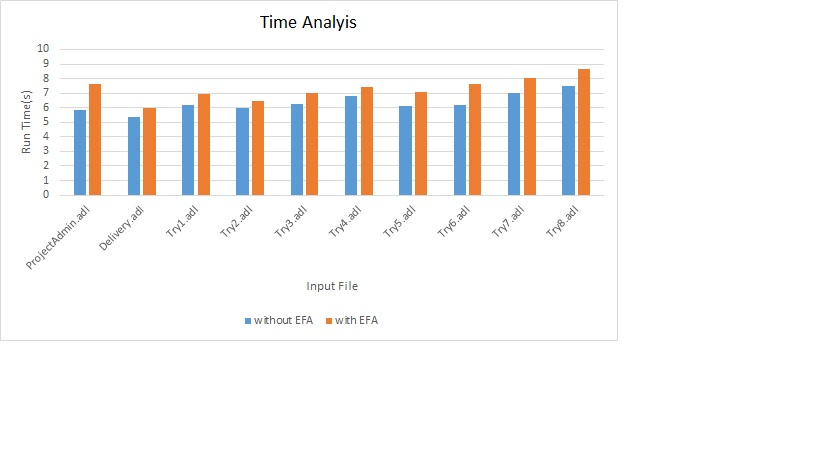
\includegraphics[width=1.3\textwidth]{../Chart1}
\caption{Run Time chart for test case 1 to 10.}~\label{fig:figure1}
\end{figure}


\begin{figure}
  \centering
%    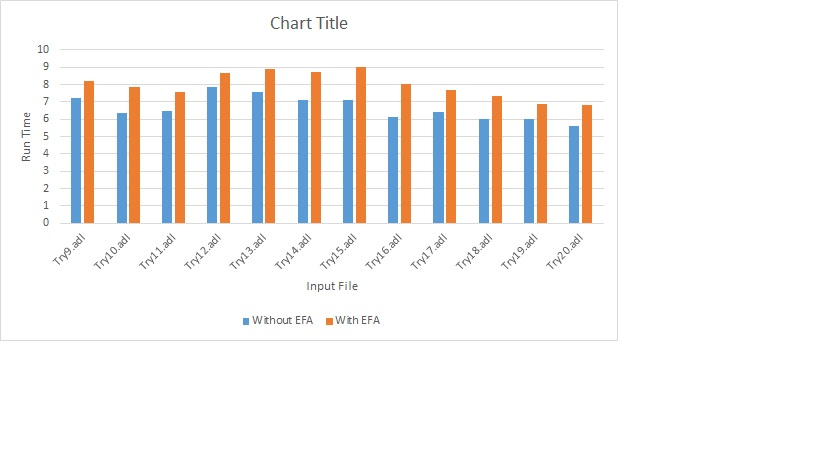
\includegraphics[width=1.3\textwidth]{../Chart2}
\caption{Run Time chart for test case 11 to 22.}~\label{fig:figure2}
\end{figure}

After measuring the performance of the current version of Ampersand compared to the EFA project we found out that there is a overhead cost of generating SQL statements from the ECA rules. The average overhead time of running EFA project is 1.16 sec. 

Calculate using the formula : 
\begin{equation}
	Overhead Time(s) =\frac{\left ( \sum  Run Time with EFA - Run Time without EFA\right )}{ No. of Test Cases}
\end{equation}

Figure\ref{fig:figure1} and Figure\ref{fig:figure2} shows a comparison of running time for all the test cases. The overhead cost of integrating EFA into Ampersand will add roughly about 1 second to the time it takes to generate a prototype. However the overall running time is still under 9 seconds for all the test cases so the waiting time for the end user is still very small compared to cost and time required to create an information system otherwise.

%%%%%%%%%%%%%
\subsection{Robustness}
The language dependency of using Haskell for this project allows the Developers to pattern match against all possible inputs. The Project was tested using the `' - -Wall'' flag to turn on all the warning options in Haskell. This allowed the team to pattern match against all possible inputs, this way the project does not rely on the test cases reachable through the Ampersand test input files. 

%%%%%%%%%%%%%%%%%%%%%%%%%%%%%SECTION: UNIT TESTS %%%%%%%%%%%%%%%%%%%%%%%%%%%%%%%
\section{EFA Tests}
Disclaimer: Although some functions were unit tested, the types used as inputs 
for those functions were not individually tested. We have assumed that the 
types of data used in these tests are correct if the tests pass and the 
functions work as intended. The passed tests matches the output type with the 
expected output type.
\subsection{Unit Tests}
These tests compared function output and expected output, readProcess was used 
to read the output of these function. If assumptions were correct, returned 
type should be equivalent to expected type. When these modules are compiled and 
the functions are called, the cabal system also tests for type correctness. 
Correctness is assumed from type correctness, and the types are identified by 
their associated properties. Lastly, the tests that failed due to in the input 
of false parameters or breaking restrictions placed on the data types were 
excluded from the tests because they do not speak to the correctness of these 
functions and were caused by human error.\\
\begin{adjustwidth}{-0.5cm}{}

\begin{tabular}[h!]{ |p{5cm}||p{3cm}|p{3cm}|p{3cm}|  }
    
    \hline
    \multicolumn{4}{|c|}{Utils.hs} \\
    \hline
    Function Name & Tests Passed & Tests Failed & Success Rate\\
    \hline
    prod2sing   & 5    &0&   100\\
    sing2prod&   5  & 0   &100\\
    foldrProd &5 & 0&  100\\
    foldlProd &5 & 0&  100\\
    mapProd&   5  & 0&100\\
    someProd& 5  & 0   &100\\
    compareSymbol& 5  & 0&100\\
    neq\_is\_neq& 5  & 0&100\\
    not\_equal\_does\_not\_reduce& 5  & 0&100\\
    is\_falsum& 5  & 0&100\\
    openSetRec& 5  & 0&100\\
    openNotElem& 5  & 0&100\\
    decNotElem& 5  & 0&100\\
    decSetRec& 5  & 0&100\\
    lookupRecM& 5  & 0&100\\
    lookupRec& 5  & 0&100\\
    unzipRec& 5  & 0&100\\
    recAssocs& 5  & 0&100\\
    recLabels& 5  & 0&100\\
    if\_pure& 5  & 0&100\\
    if\_ap& 5  & 0&100\\
    freshNames& 5  & 0 &100\\
    \hline
\end{tabular}

\end{adjustwidth}

\begin{adjustwidth}{-0.5cm}{}    
    \begin{tabular}[h!]{ |p{5cm}||p{3cm}|p{3cm}|p{3cm}|  }
        
        \hline
        \multicolumn{4}{|c|}{TypedSQL.hs} \\
        \hline
        Function Name & Tests Passed & Tests Failed & Success Rate\\
        \hline
        isScalarType   & 5    &0&   100\\
        isScalarTypes&   5  & 0   &100\\
        typeOf &5 & 0&  100\\
        argOfRel &5 & 0&  100\\
        typeOfSem&   5  & 0&100\\
        colsOf& 5  & 0   &100\\
        unsafeSQLValFromName& 5  & 0&100\\
        unsafeSQLValFromQuery& 5  & 0&100\\
        unsafeSQLValFromQuery& 5  & 0&100\\
        unsafeRefFromName& 5  & 0& 100\\
        deref& 5  & 0&100\\
        typeOfTableSpec& 5  & 0&100\\
        typePfTableSpec'& 5  & 0&100\\
        tableSpec& 5  & 0&100\\
        someTableSpec& 5  & 0&100\\
        lookupRec& 5  & 0&100\\
        \hline
    \end{tabular}
\end{adjustwidth}

\begin{adjustwidth}{-0.5cm}{}    
    \begin{tabular}[h!]{ |p{5cm}||p{3cm}|p{3cm}|p{3cm}|  }
        
        \hline
        \multicolumn{4}{|c|}{TSQLCombinators.hs} \\
        \hline
        Function Name & Tests Passed & Tests Failed & Success Rate\\
        \hline
        primSQL   & 10  & 0&   100\\
        sql       & 10  & 0&   100\\
        \hline
    \end{tabular}
\end{adjustwidth}

\begin{adjustwidth}{-0.5cm}{}    
    \begin{tabular}[h!]{ |p{5cm}||p{3cm}|p{3cm}|p{3cm}|  }
        
        \hline
        \multicolumn{4}{|c|}{Trace.hs} \\
        \hline
        Function Name & Tests Passed & Tests Failed & Success Rate\\
        \hline
        takePrefix   & 10    &0&   100\\
        getTraceInfo&   10  & 0   &100\\
        impossible & 10 & 0&  100\\
        \hline
    \end{tabular}
\end{adjustwidth}

\begin{adjustwidth}{-0.5cm}{}    
    \begin{tabular}[h!]{ |p{5cm}||p{3cm}|p{3cm}|p{3cm}|  }      
        \hline
        \multicolumn{4}{|c|}{Singletons.hs} \\
        \hline
        Function Name & Tests Passed & Tests Failed & Success Rate\\
        \hline
        withSingT   & 5    &0&   100\\
        withSingW&   5  & 0   &100\\
        witness &5 & 0&  100\\
        singKindWitness1 &5 & 0&  100\\
        singKindWitness2 &   5  & 0&100\\
        sing2val & 5  & 0   &100\\
        val2sing& 5  & 0&100\\
        tyRepOfW& 5  & 0&100\\
        eqSymbol& 5  & 0&100\\
        eqProdTypRep& 5  & 0& 100\\
        elimSingT& 5  & 0&100\\
        (\%==) & 5  & 0&100\\
        \hline
    \end{tabular}
\end{adjustwidth}

\begin{adjustwidth}{-0.5cm}{}    
    \begin{tabular}[h!]{ |p{5cm}||p{3cm}|p{3cm}|p{3cm}|  }
        
        \hline
        \multicolumn{4}{|c|}{Equality.hs} \\
        \hline
        Function Name & Tests Passed & Tests Failed & Success Rate\\
        \hline
        doubleneg   & 3    &0&   100\\
        triviallyTrue &   3  & 0   &100\\
        mapNeg & 3 & 0&  100\\
        elimNeg & 3 & 0&  100\\
        mapDec  &   3  & 0&100\\
        liftDec2 & 3  & 0   &100\\
        dec2bool & 3  & 0& 100\\
        \hline
    \end{tabular}
\end{adjustwidth}
%%%%%%%%%%%%%%%%%%%%%%%%%%%%%SECTION: BLACKBOX TEST %%%%%%%%%%%%%%%%%%%%%%%%%%%%
\subsection{Randomized Testing}
QuickCheck is a  testing tool that uses type-based testing, it uses invariants 
to check for specific properties that should be retained in a purely functional 
program such as idempotency, where applying a function twice has the same 
result as applying it only once. QuickCheck generates tests data and passes it 
to the property chosen by the user; the type of property determines which data 
generator can be used. Each of the tests for functions are usually prefixed 
with \textit{prop\_} to distinguish them from the real functions. For functions 
that are similar to build in functions. If a function is similar in behaviour 
to a build-in function, testing against the model (i.e., the build-in function) 
can be done to validate its correctness, but that is not used here due to the 
unique properties of these functions which could not be easily decomposed into 
simpler forms.
\begin{adjustwidth}{-0.5cm}{}   
\begin{tabular}[h!]{ |p{5cm}||p{3cm}|p{3cm}|p{3cm}|  }
    \hline
    \multicolumn{4}{|c|}{Utils.hs} \\
    \hline
    Function Name & Tests Passed & Tests Failed & Success Rate\\
    \hline
    prod2sing   & 100    &0&   100\\
    sing2prod&   100  & 0   &100\\
    foldrProd &100 & 0&  100\\
    foldlProd &100 & 0&  100\\
    mapProd&   100  & 0&100\\
    someProd& 100  & 0   &100\\
    compareSymbol& 100  & 0&100\\
    neq\_is\_neq& 100  & 0&100\\
    not\_equal\_does\_not\_reduce& 100  & 0&100\\
    is\_falsum& 100  & 0&100\\
    openSetRec& 100  & 0&100\\
    openNotElem& 100  & 0&100\\
    decNotElem& 100  & 0&100\\
    decSetRec& 100  & 0&100\\
    lookupRecM& 100  & 0&100\\
    lookupRec& 100  & 0&100\\
    unzipRec& 100  & 0&100\\
    recAssocs& 100  & 0&100\\
    recLabels& 100  & 0&100\\
    if\_pure& 100  & 0&100\\
    if\_ap& 100  & 0&100\\
    freshNames& 100  & 0 &100\\
    \hline
\end{tabular}
\end{adjustwidth}

\begin{adjustwidth}{-0.5cm}{}    
    \begin{tabular}[h!]{ |p{5cm}||p{3cm}|p{3cm}|p{3cm}|  }
        
        \hline
        \multicolumn{4}{|c|}{TypedSQL.hs} \\
        \hline
        Function Name & Tests Passed & Tests Failed & Success Rate\\
        \hline
        isScalarType   & 100    &0&   100\\
        isScalarTypes&   100  & 0   &100\\
        typeOf &100 & 0&  100\\
        argOfRel &100 & 0&  100\\
        typeOfSem&   100  & 0&100\\
        colsOf& 100  & 0   &100\\
        unsafeSQLValFromName& 100  & 0&100\\
        unsafeSQLValFromQuery& 100  & 0&100\\
        unsafeSQLValFromQuery& 100  & 0&100\\
        unsafeRefFromName& 100  & 0& 100\\
        deref& 100  & 0&100\\
        typeOfTableSpec& 100  & 0&100\\
        typePfTableSpec'& 100  & 0&100\\
        tableSpec& 100  & 0&100\\
        someTableSpec& 100  & 0&100\\
        lookupRec& 100  & 0&100\\
        \hline
    \end{tabular}
\end{adjustwidth}

\begin{adjustwidth}{-0.5cm}{}    
    \begin{tabular}[h!]{ |p{5cm}||p{3cm}|p{3cm}|p{3cm}|  }
        
        \hline
        \multicolumn{4}{|c|}{TSQLCombinators.hs} \\
        \hline
        Function Name & Tests Passed & Tests Failed & Success Rate\\
        \hline
        primSQL   & 100  & 0&   100\\
        sql       & 100  & 0&   100\\
        \hline
    \end{tabular}
\end{adjustwidth}

\begin{adjustwidth}{-0.5cm}{}    
    \begin{tabular}[h!]{ |p{5cm}||p{3cm}|p{3cm}|p{3cm}|  }
        
        \hline
        \multicolumn{4}{|c|}{Trace.hs} \\
        \hline
        Function Name & Tests Passed & Tests Failed & Success Rate\\
        \hline
        takePrefix   & 100    &0&   100\\
        getTraceInfo&   100  & 0   &100\\
        impossible & 100 & 0&  100\\
        \hline
    \end{tabular}
\end{adjustwidth}

\begin{adjustwidth}{-0.5cm}{}    
    \begin{tabular}[h!]{ |p{5cm}||p{3cm}|p{3cm}|p{3cm}|  }      
        \hline
        \multicolumn{4}{|c|}{Singletons.hs} \\
        \hline
        Function Name & Tests Passed & Tests Failed & Success Rate\\
        \hline
        withSingT   & 100    &0&   100\\
        withSingW&   100  & 0   &100\\
        witness &100 & 0&  100\\
        singKindWitness1 &100 & 0&  100\\
        singKindWitness2 &   100  & 0&100\\
        sing2val & 100  & 0   &100\\
        val2sing& 100  & 0&100\\
        tyRepOfW& 100  & 0&100\\
        eqSymbol& 100  & 0&100\\
        eqProdTypRep& 100  & 0& 100\\
        elimSingT& 100  & 0&100\\
        (\%==) & 100  & 0&100\\
        \hline
    \end{tabular}
\end{adjustwidth}

\begin{adjustwidth}{-0.5cm}{}    
    \begin{tabular}[h!]{ |p{5cm}||p{3cm}|p{3cm}|p{3cm}|  }
        
        \hline
        \multicolumn{4}{|c|}{Equality.hs} \\
        \hline
        Function Name & Tests Passed & Tests Failed & Success Rate\\
        \hline
        doubleneg   & 100    &0&   100\\
        triviallyTrue &   100  & 0   &100\\
        mapNeg & 100 & 0&  100\\
        elimNeg & 100 & 0&  100\\
        mapDec  &   100  & 0&100\\
        liftDec2 & 100  & 0   &100\\
        dec2bool & 100  & 0& 100\\
        \hline
    \end{tabular}
\end{adjustwidth}

%%%%%%%%%%%%%%%%%%%%%%%%%%%%%SECTION: SQL CORRECTNESS%%%%%%%%%%%%%%%%%%%%%%%%%%%
\subsection{SQL Output Tests}
Workbench was used to test the syntactic correctness of SQL queries. The same 
scripts will repeated generate the exact same SQL queries, only two cycles of 
tests have been completed but both produce identical results.\\
\begin{figure}[H]

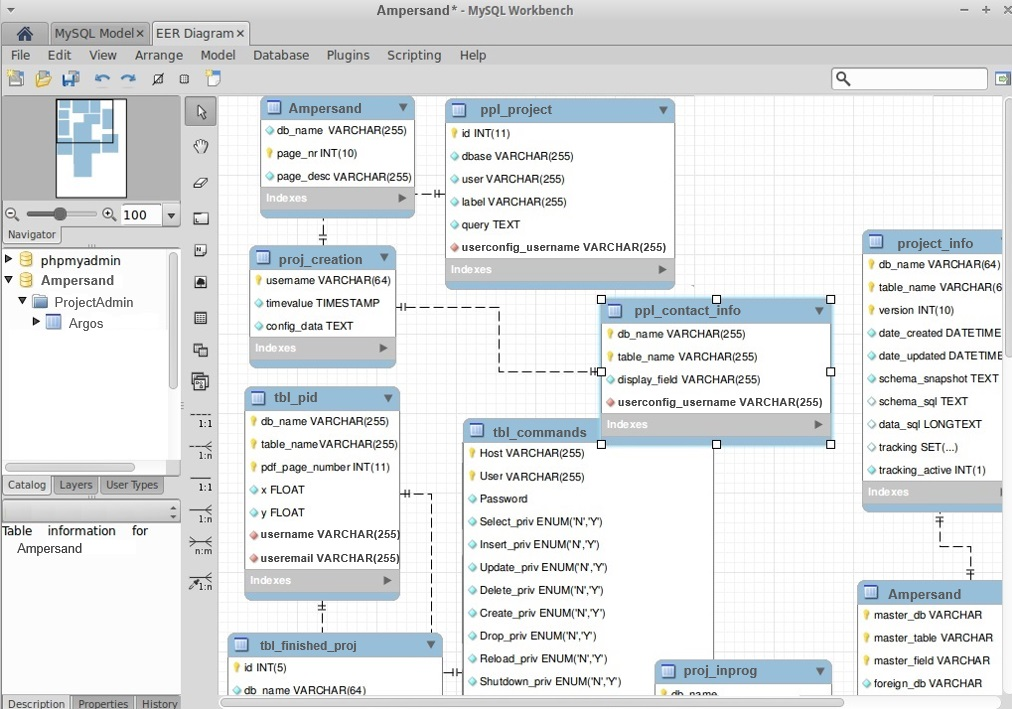
\includegraphics[width=\textwidth]{workbench_linux}
\caption{This is an example of what Workbench looks like using ProjectAdmin as 
    the prototype}
\end{figure}
\begin{adjustwidth}{-0.5cm}{}   
    \begin{tabular}[h!]{ |p{5cm}||p{3cm}|p{3cm}|p{3cm}|  }
        \hline
        \multicolumn{4}{|c|}{Generated SQL Test Table} \\
        \hline
        Test Script (.adl) & SQL Accepted & Number of Tries & Success Rate\\
        \hline
        ProjectAdmin & Yes    &2&   100\\
        Delivery&   Yes  & 2   &100\\
        Try1 &Yes & 2&  100\\
        Try2 &Yes & 2&  100\\
        Try3&   Yes  & 2&100\\
        Try4& Yes  & 2   &100\\
        Try5& Yes  & 2&100\\
        Try6& Yes  & 2&100\\
        Try7& Yes  & 2&100\\
        Try8& Yes  & 2&100\\
        Try9& Yes  & 2&100\\
        Try10& Yes  & 2&100\\
        Try11& Yes  & 2&100\\
        Try12& Yes  & 2&100\\
        Try13& Yes  & 2&100\\
        Try14& Yes  & 2&100\\
        Try15& Yes  & 2&100\\
        Try16& Yes  & 2&100\\
        Try17& Yes  & 2&100\\
        Try18& Yes  & 2&100\\
        Try19& Yes  & 2&100\\
        Try20& Yes  & 2 &100\\
        \hline
    \end{tabular}
\end{adjustwidth}

%%%%%%%%%%%%%%%%%%%%%%%%%%%%%SECTION: SQL CORRECTNESS%%%%%%%%%%%%%%%%%%%%%%%%%%%
\section{System Tests}
In this section we document the result of parsing ADL files through the EFA project.   

\subsection {Testing Issues}
Imported data structures were assumed to be correct from the original Ampersand 
design because they have been through rigorous testing. The data structures 
that were created specifically to represent SQL data structures were assumed to 
be correct if the generated SQL queries was not rejected by the test database. 
The cabal systems assures semantic correctness when these programs are compiled 
or otherwise it would not run, thus no further was testing was done on this 
front.

\subsection{Ampersand generates ASQL}
\begin{longtable}{|L{0.5cm}|L{2.5cm}|L{2.5cm}|L{2.25cm}|L{3cm}|L{1.75cm}|L{1.5cm}|}
\hline
\textbf{No.} & \textbf{Test Case}  & \textbf{Initial State} & \textbf{Input} & \textbf{Expected Output} & \textbf{Actual Output} & \textbf{Result}\\ 
\hline
1 & Ampersand generates ASQL & Installed EFA Ampersand &ProjectAdmin.adl & Annotated SQL & As Expected & PASS \\ 
\hline
2 & Ampersand generates ASQL & Installed EFA Ampersand &Delivery.adl & Annotated SQL & As Expected & PASS \\ 
\hline
3 &Ampersand generates ASQL & Installed EFA Ampersand &Case.adl & Annotated SQL & As Expected & PASS \\ 
\hline
\end{longtable}

\subsection{ASQL is valid}
\begin{longtable}{|L{0.5cm}|L{2.5cm}|L{2.5cm}|L{2.25cm}|L{3cm}|L{1.75cm}|L{1.5cm}|}
\hline
%\textbf{No.} & \textbf{Test Case}  & \textbf{Initial State} & \textbf{Input} & \textbf{Expected Output} & \textbf{Actual Output} & \textbf{Result}\\ 
%\hline
%1 & Ampersand generates ASQL & Installed EFA Ampersand &ProjectAdmin.adl & Annotated SQL & As Expected & PASS \\ 
%\hline
%2 & Ampersand generates ASQL & Installed EFA Ampersand &Delivery.adl & Annotated SQL & As Expected & PASS \\ 
%\hline
%3 &Ampersand generates ASQL & Installed EFA Ampersand &Case.adl & Annotated SQL & As Expected & PASS \\ 
%\hline
\end{longtable}

\subsection{EFA System Compatibility}
\begin{longtable}{|L{0.5cm}|L{2.5cm}|L{2.5cm}|L{2.25cm}|L{3cm}|L{1.75cm}|L{1.5cm}|}
\hline
\textbf{No.} & \textbf{Test Case}  & \textbf{Initial State} & \textbf{Input} & \textbf{Expected Output} & \textbf{Actual Output} & \textbf{Result}\\ 
\hline
1 & System Compatibility & Installed EFA Ampersand &ProjectAdmin.adl & No exception during generation of prototype & As Expected & PASS \\ 
\hline
2 & System Compatibility & Installed EFA Ampersand &Delivery.adl & No exception during generation of prototype & As Expected & PASS \\ 
\hline
3 & System Compatibility & Installed EFA Ampersand &Case.adl & No exception during generation of prototype & As Expected & PASS \\ 
\hline
\end{longtable}

\subsection{EFA is a pure function}
Since all functions written in
Haskell are pure, and the  Haskell type checker accepts our program hence the test is passed.

\subsection{EFA gives appropiate feedback}
This feature will be implemented on the front-end after integration into the core Ampersand project. When the prototype is run, and a violation occurs, the resulting output will look like :

\begin{verbatim}
======= Violation log entry <...>
=== ECA rule fired: <...> 
=== Delta: <...>
=== Original rule: cast;instantiates |- qualifies;comprises~
Violation occurred because rule "who's cast in roles" was not 
 satisfied. This is because "an Actor may appear in a 
 Performance of the Play only if the Actor is skilled for a 
 Role that the Play comprises"
\end{verbatim}

\subsection{EFA code walk-through}
With reference to T9 test in the test report (see page 19 of the test plan). EFA team will be doing a code walk-through with the product owners. This walk-through is not scheduled at this point. The Ampersand Team will be invited to attend the final demonstration which is to be scheduled in April.

\subsection{Sentinel Test}
After review and acceptance of the EFA project. EFA will be ran on the sentinel (see test case T13 on page 18 of Test Plan). The sentinel test is performed at regular intervals and emails developers about any failed test. This will serve as automated testing of EFA project in the future.

%%%%%%%%%%%%%%%%%%%%%%%%%%%%%
%%%%%%%%%%%%%%%%%%%%%%%%%%%%%
\section{Changes Made After testing}
After intense usability testing, the EFA team decided to format the generated SQL using a pretty printer library. The formatted SQL is indented for better readability and thereby increasing the overall usability of the EFA project.

\bibliographystyle{alpha}
\bibliography{}

\end{document}

%%  LocalWords:  UML
